\chapter{Testing}

\section{Overall Approach to Testing}

This chapter presents a multitude of different testing types. There are automated unit tests to ensure the internal code logic behaves as expected. The User Interface tests are tests which are difficult to automate but are used to ensure that the user interface models the correct state of execution. Acceptance testing is used to assess how well the applications meets the specified requirements in section \ref{funcymcdunky}. Stress testing has been considered by the author but ultimately has been omitted. The author feels that the application is never subject to heavy loads, nor can the user exceed the normal operational load for the application. Overall the testing process is not as thorough as the author desires however, given the short time frame for the projects development the author feels that the testing suffices in ensuring correct functionality.

\section{White-box Testing}
\subsection{Unit Tests}

There are features present in the application code which the author has excluded from the unit testing process. Any feature which relies on random numbers to perform its task has not been unit tested. The author feels that any methods which uses a random number can’t reliably be tested therefore, it doesn’t makes sense to attempt to. Instead the author has extracted the code which relies on such random numbers and tested the behaviour of such code using specifically defined values, this enables the author to accurately test for expected behaviours. In addition to this getter and setter methods or simple assignment operations have not been tested. The reason for excluding these methods from unit tests is because the code responsible is so simple it can’t realistically fail so there is no real purpose in producing such tests.

The unit tests that the author has produced revolve around ensuring that only legal algorithm parameters are accepted and that the movement, probability and pheromone functions are behaving as expected and return legal values. These tests contain validation checks against a range of values for each parameter including boundary conditions to ensure that they are correctly dealt with, examples of such testing can be seen in figures \ref{testAlpha} to \ref{testProb}. There are many more tests present in the test package for the application however the author has only briefly outlined a small number of these. Evidence of such testing can be seen below in figure \ref{testSS}.

\begin{figure}[H]
\centering
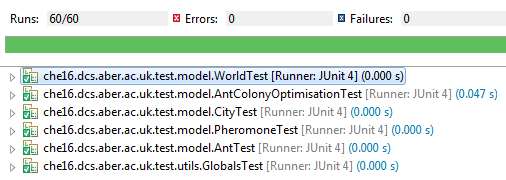
\includegraphics[scale=0.8]{Images/chapter6/testSS}
\caption[Unit Testing Summary]{Evidence of the completed execution of the applications unit tests. The view present is the built in Eclipse JUnit interface.}
\label{testSS}
\end{figure}

\section{Black-box Testing}
\subsection{User Interface Testing}

It is difficult to reliably test the graphical user interface using a white-boxing testing approach. To overcome this obstacle the author has decided to manually test the user interface using a black-box testing approach to ensure the correct behaviour is exhibited. During this test process the author did not repeat any test previously executed in the unit testing process.

The file IO process will also be tested to ensure that configurations can be correctly loaded and saved to a specified file. Several test files will be produced, each file will be designed to test a variety of possible legal and illegal file contents. Tests will be done to ensure that the application rejects files that contain; missing data, incorrect type for a specified value and city coordinates which exceeds the bounds of the canvas. The saving of a configuration to a file doesn’t not need to be as rigorously tested as the algorithm has to be instantiated with legal values before the writing process can be executed therefore, the values of the written file will be legal and of the correct format. An example of such file contents can be found in appendix D, section \ref{fileIOtest}. The full list of black-box tests performed by the author can be seen in section appendix D, section \ref{UITESTSM8}.

\subsection{Acceptance Testing}

Due to the lack of a dedicated client acceptance testing proved difficult for this project. For the purpose of these acceptance tests the author acted as the end user, and used the application in a non-bias manner and adapted the mind-set of a new user. This is far from an ideal way to perform acceptance tests and this process isn’t truly representative of real acceptance testing. The application itself is not a finished deployment ready product. Before this would be the case the author would like to extend current functionality and provide a larger variety of algorithm types and modifiers. If the author had a larger time frame then a distinct customer or user group would be set up to ensure this acceptance testing process is performed to the highest quality. Similar tests have been grouped together, the results of this process can be found in appendix D, \ref{AcceptanceTestz}.